% ============================================================================
%  VagueAider -- User Study (user-friendliness, vagueness, instruction habits)
%  Paper-ready LaTeX. Two ways to use this file:
%    (1) Compile standalone:  pdflatex user_study.tex
%    (2) Drop into your paper: copy everything between the two
%        "%% >>> BODY" / "%% <<< BODY" markers, and make sure the preamble
%        packages below are present. Figures are referenced relative to this
%        directory (set \graphicspath if you move the .tex).
% ============================================================================
\documentclass[11pt]{article}
\usepackage[margin=1in]{geometry}
\usepackage{graphicx}
\usepackage{booktabs}
\usepackage{tabularx}
\usepackage{array}
\usepackage{amssymb}
\usepackage{xcolor}
\usepackage{caption}
\usepackage{mdframed}
\usepackage[hidelinks]{hyperref}

\graphicspath{{.}{./}}            % PNGs live next to this .tex
\newcolumntype{Y}{>{\raggedright\arraybackslash}X}
\newcommand{\pct}{\%}
\definecolor{ufgreen}{HTML}{2A9D8F}
\definecolor{afred}{HTML}{E76F51}

% Light-grey framed box for the questionnaire (Appendix B); breaks across pages.
\mdfdefinestyle{qbox}{%
  backgroundcolor=black!4, linecolor=black!35, linewidth=0.6pt, roundcorner=2pt,
  innertopmargin=9pt, innerbottommargin=10pt, innerleftmargin=11pt,
  innerrightmargin=11pt, skipabove=6pt, skipbelow=6pt}
% question stem (bold) + choice-type tag (grey italic)
\newcommand{\qq}[2]{\noindent\textbf{#1} {\itshape\footnotesize\color{black!55}(#2)}\par\nobreak\smallskip}

\title{\vspace{-2em}User Study: User-Friendly Vague Intents vs.\ Agent-Friendly Executable Instructions}
\author{}
\date{}

\begin{document}
\maketitle

%% >>> BODY ===================================================================

\section{User Study}
\label{sec:userstudy}

\paragraph{Motivation and design.}
The central premise of VagueAider is that real users express their needs as
\emph{user-friendly vague intents}, whereas a mobile agent requires
\emph{agent-friendly executable instructions}, and that a \emph{semantic gap}
separates the two. To check that this gap is felt by users rather than being an
artifact of our benchmark, we ran a $7$-item questionnaire on smartphone
AI-assistant usage and instruction habits, collecting $n{=}28$ valid responses
(two background items, two multi-select diagnostic items, and three
single-select items probing instruction granularity). The full translated
instrument and per-option counts are given in Appendix~\ref{app:survey}.

\paragraph{Definitions.}
We treat the two notions as the two ends of a single \emph{granularity axis}:
\begin{itemize}
  \item \textbf{User-friendliness} -- how closely an instruction matches the way
  a person naturally voices intent, i.e.\ the articulation/cognitive cost the
  user pays. A highly user-friendly instruction states only the \emph{final
  goal} and leaves the choice of app and the concrete steps to the system
  (e.g.\ \textit{``Buy me the cheapest Switch controller.''}).
  \item \textbf{Agent-friendliness} -- how directly executable an instruction is
  for the agent: an explicit target app and atomic, UI-level steps that require
  no inference (e.g.\ \textit{``Open Taobao, tap the search box, type `Switch
  controller', sort by price ascending, pick the first\,\ldots''}).
\end{itemize}
VagueBench discretizes this axis into three ambiguity levels
(Table~\ref{tab:levels}); survey item Q5 instantiates the same axis on a single
shopping task as options A (user-friendly), B (benchmark-style: names apps but
leaves the operations to the agent) and C (agent-friendly).

\begin{table}[t]
  \centering
  \caption{Ambiguity levels in VagueBench. Each level removes a different piece
  of the information an agent would need to act.}
  \label{tab:levels}
  \small
  \begin{tabularx}{\linewidth}{@{}l l Y l@{}}
    \toprule
    \textbf{Level} & \textbf{Name} & \textbf{Missing information} & \textbf{Example} \\
    \midrule
    L1 & Implicit App & Action is clear; the target app is unspecified & \textit{``Order a spicy pizza.''} \\
    L2 & Implicit Op  & The app is named; the concrete steps are missing & \textit{``Use Uber to go to the airport.''} \\
    L3 & Fully Vague  & Only the core need is expressed & \textit{``I want to watch a movie.''} \\
    \bottomrule
  \end{tabularx}
\end{table}

\paragraph{Sample.}
Usage frequency (Q1) spans the spectrum: several times a week 46.4\pct,
multiple times a day 21.4\pct, $1$--$2$ times a day 7.1\pct, and almost
never 25.0\pct. On awareness of screen-operating next-generation agents (Q2),
64.3\pct have heard of but not deeply used such systems and 17.9\pct follow
them closely, so most respondents understand the paradigm without being
habituated to a particular product---their stated preferences reflect
expectations of an ideal agent rather than accommodation to an existing tool.

\subsection{Today's pain points and tomorrow's expectations (Q3, Q4)}

Figure~\ref{fig:problems} pairs the most-cited pain points of current assistants
(Q3) with the most-wanted future capabilities (Q4). Strikingly, the top two
answers to \emph{both} questions are exactly the two capabilities VagueAider
targets. The leading complaints are the inability to complete cross-app tasks
(71.4\pct) and the inability to understand abstract ideas without rigid,
step-by-step commands (64.3\pct)---ahead of speed (28.6\pct), battery
(32.1\pct), and even privacy (42.9\pct). Symmetrically, the most-desired
capabilities are smooth cross-app coordination (82.1\pct) and strong
abstract-intent understanding (64.3\pct, tied with privacy). In other words,
\emph{understanding vague intent and acting across apps} is simultaneously the
largest source of dissatisfaction and the strongest demand---empirically
grounding the problem VagueBench measures and VagueAider addresses.

\begin{figure}[t]
  \centering
  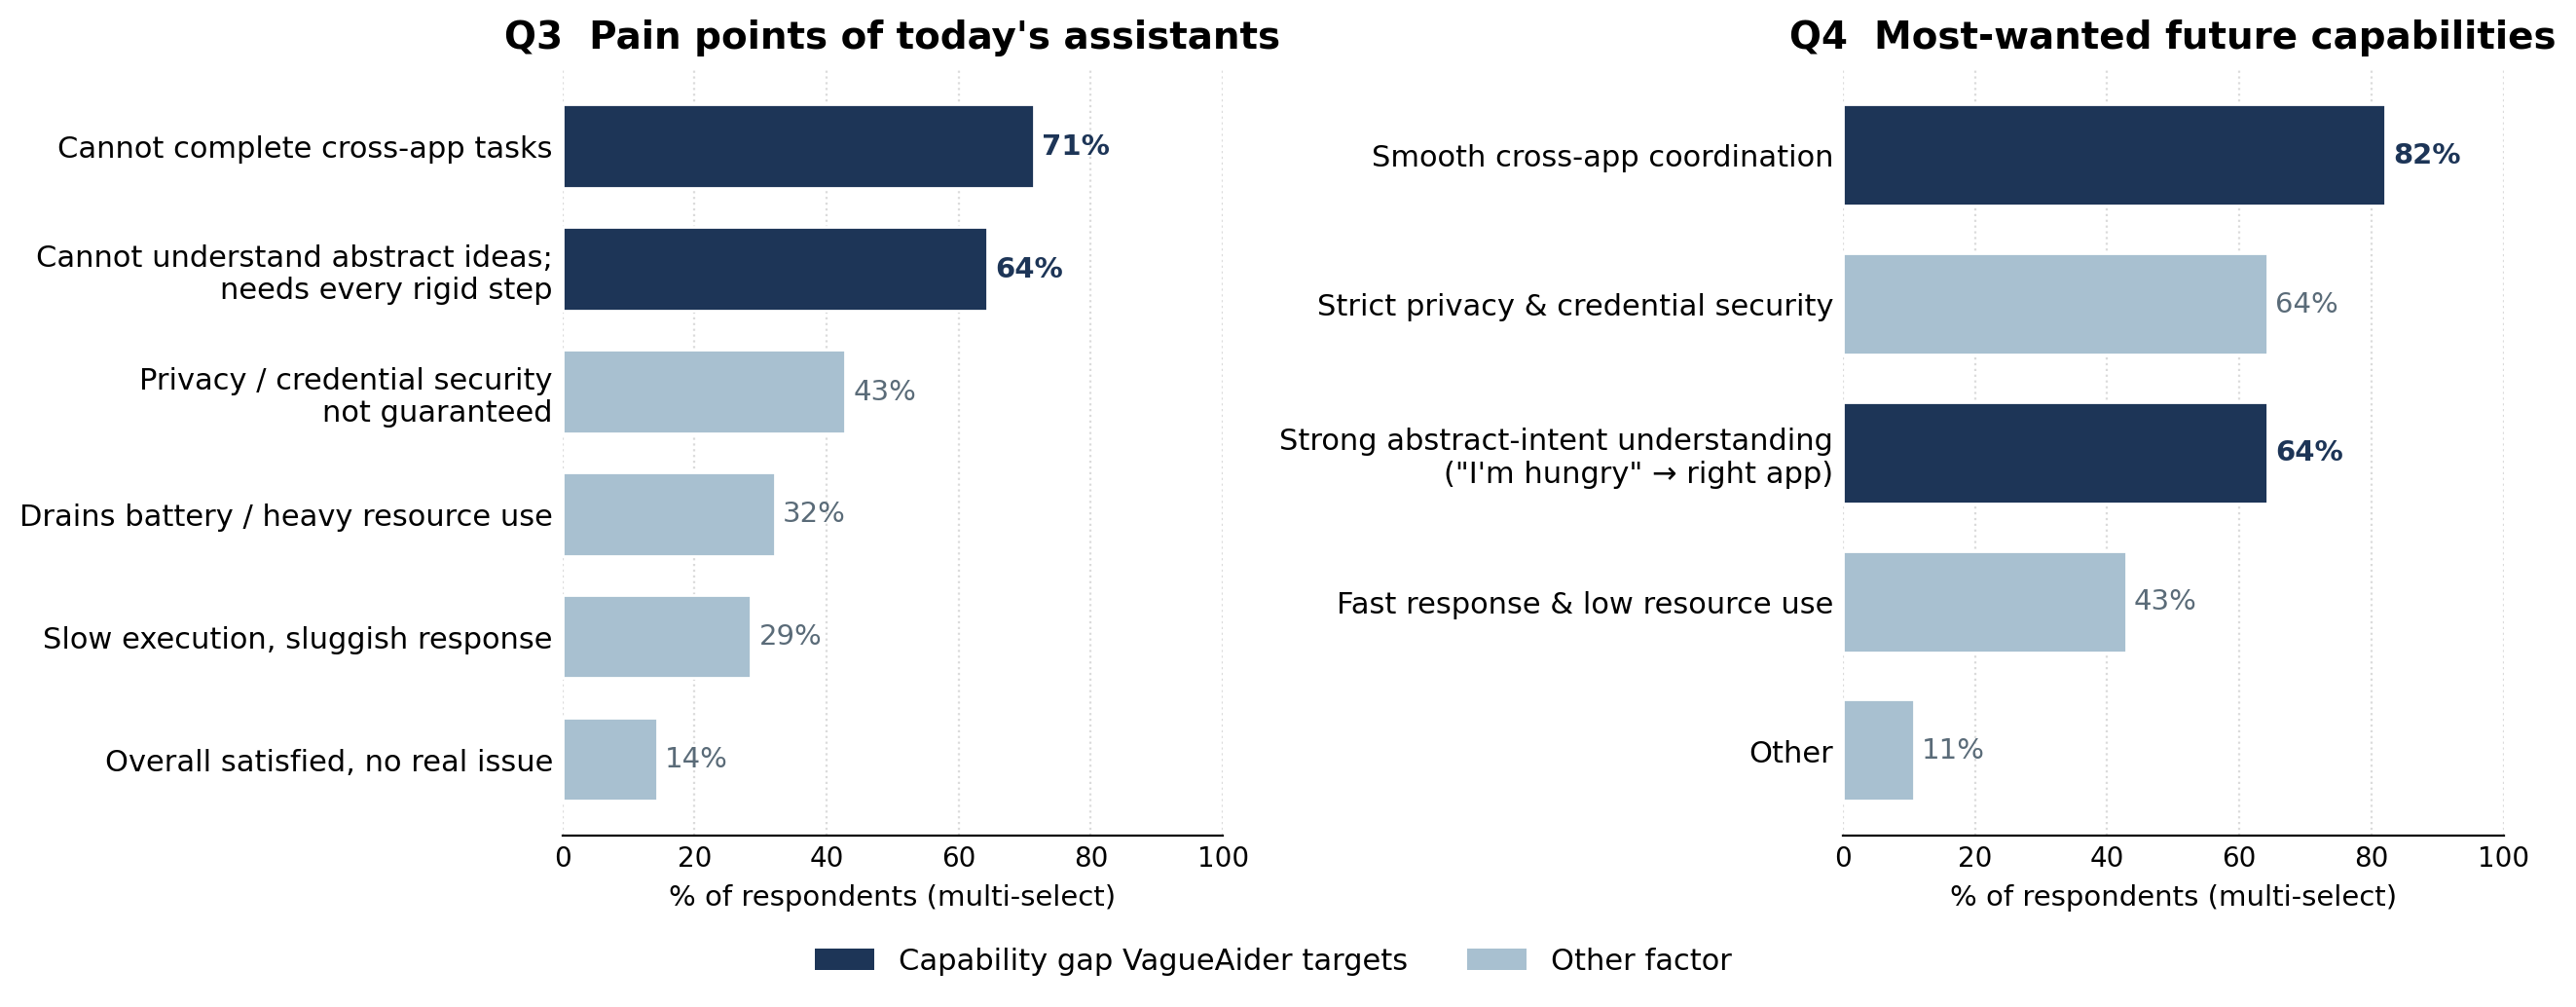
\includegraphics[width=\linewidth]{fig_survey_problems.png}
  \caption{Q3 (pain points of today's assistants) and Q4 (most-wanted future
  capabilities), both multi-select, $n{=}28$. Bars in dark navy mark the two
  capability gaps VagueAider targets; they rank first and second on both
  questions.}
  \label{fig:problems}
\end{figure}

\subsection{The user-friendly $\leftrightarrow$ agent-friendly preference axis (Q5--Q7)}

Figure~\ref{fig:spectrum} projects the three single-select items onto one shared
stance axis (green: most user-friendly answer---state the vague intent and
expect the agent to bridge the gap; gray: intermediate---some detail given, but
the operations are still left to the agent; red: most agent-friendly answer---
willing to spell out every app and click).

\begin{itemize}
  \item \textbf{Q5 (how much to specify).} This item should \emph{not} be read
  as a satisfaction ranking of the three options. The medium option B (50.0\pct)
  is precisely the \emph{benchmark-style} instruction---it names apps but leaves
  the operations to the agent---yet \emph{half} the respondents (A+C, 50.0\pct)
  did \emph{not} choose it, i.e.\ about half do not treat benchmark-style
  phrasing as their preferred input. Among those who deviate, the pull toward a
  \emph{more} user-friendly phrasing (A, 32.1\pct) is roughly $1.8\times$ the
  pull toward a \emph{more} explicit one (C, 17.9\pct). On the boundary that
  matters here, A+B (82.1\pct) leave the operations for the agent to infer and
  only C (17.9\pct) gives a directly executable instruction---so even the
  ``middle'' is itself under-specified. (A 3-point detail ladder and the ``most
  habitual'' anchor both bias toward the benchmark-style middle and understate
  the user-friendly preference.)
  \item \textbf{Q6 (is babysitter-level phrasing natural?).} 50.0\pct say it
  does not match their habits at all and 39.3\pct would only do it for very
  complex or error-prone tasks; just 10.7\pct regard giving full detail as
  normal. Thus 89.3\pct do not treat agent-friendly phrasing as their default.
  \item \textbf{Q7 (rating an agent that demands explicit steps).} 50.0\pct
  judge it ``not smart enough'' and 39.3\pct accept it only as a current
  technical limitation; only 10.7\pct prefer such full control. So 89.3\pct
  would not be satisfied with an agent that forces explicit, step-level input.
\end{itemize}

\begin{figure}[t]
  \centering
  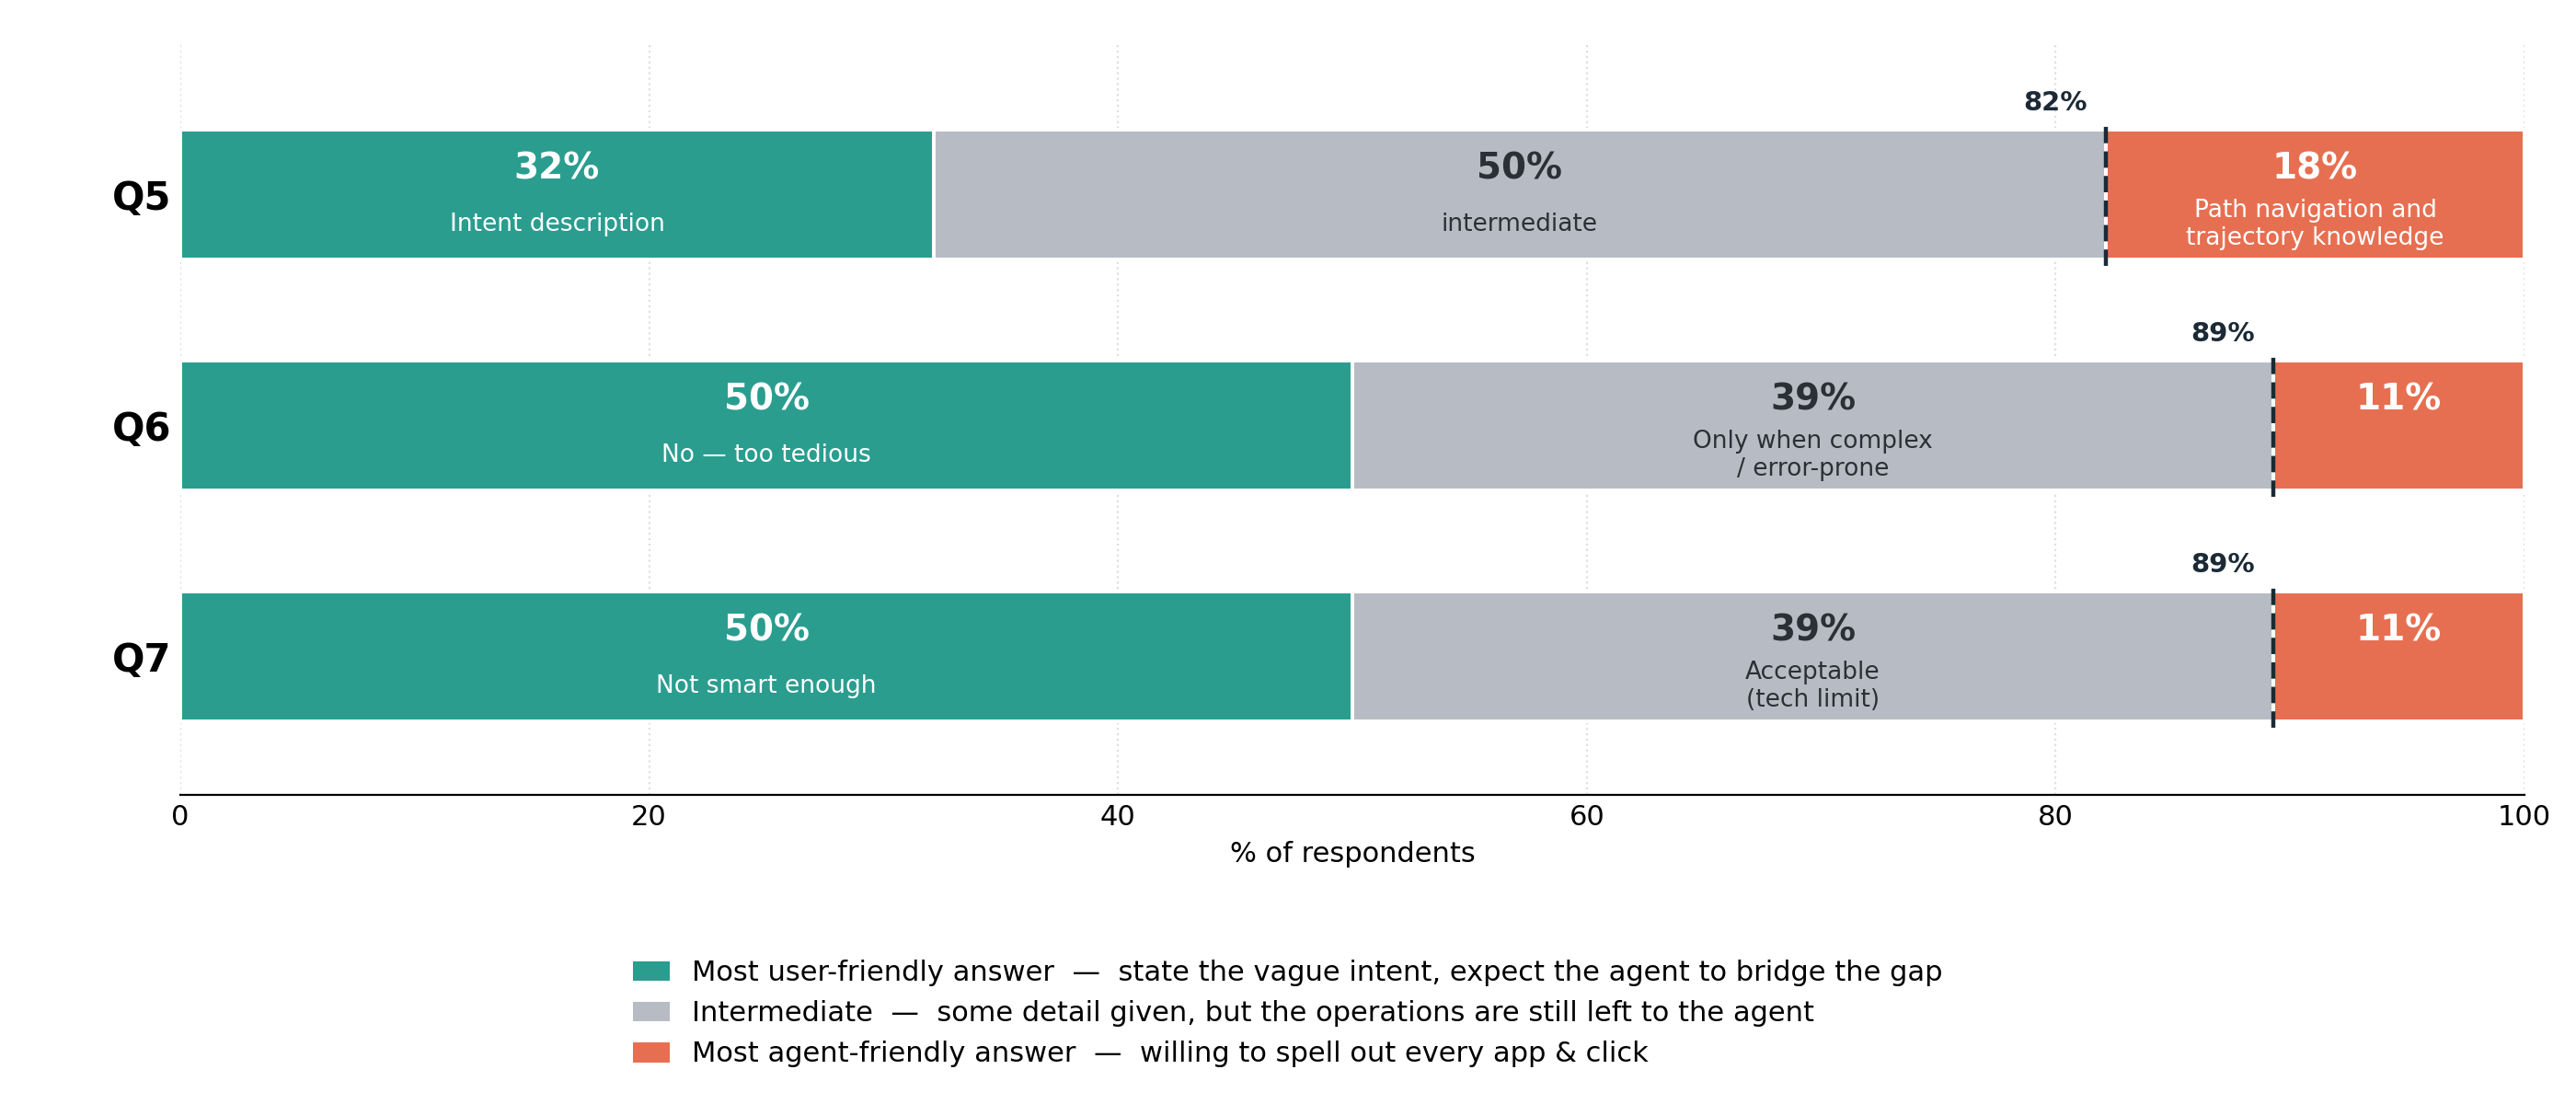
\includegraphics[width=\linewidth]{fig_survey_spectrum.png}
  \caption{Q5/Q6/Q7 (single-select, $n{=}28$) on a shared user-friendly
  $\leftrightarrow$ agent-friendly axis. Across all three items only
  11--18\pct sit at the agent-friendly (red) end; the dashed line marks the
  82--89\pct who do \emph{not} default to fully-explicit instructions.}
  \label{fig:spectrum}
\end{figure}

\begin{table}[t]
  \centering
  \caption{Q5--Q7 collapsed onto the granularity axis ($n{=}28$). For Q5 the
  intermediate column is the benchmark-style instruction (names apps, leaves
  operations to the agent), so A+B together (82.1\pct) leave the operations to
  the agent and only C (17.9\pct) is directly executable. The
  ``agent-friendly'' column is consistently small, and the recurring 89.3\pct on
  Q6/Q7 is the strongest single signal in the study.}
  \label{tab:spectrum}
  \small
  \begin{tabularx}{\linewidth}{@{}l Y c c c@{}}
    \toprule
    & \textbf{Item} & \textbf{\textcolor{ufgreen}{User-friendly}} & \textbf{Intermediate} & \textbf{\textcolor{afred}{Agent-friendly}} \\
    \midrule
    Q5 & How would you naturally phrase it?        & 32.1\pct & 50.0\pct & 17.9\pct \\
    Q6 & Is babysitter-level phrasing your habit?  & 50.0\pct & 39.3\pct & 10.7\pct \\
    Q7 & Rating an agent that needs every step     & 50.0\pct & 39.3\pct & 10.7\pct \\
    \bottomrule
  \end{tabularx}
\end{table}

\subsection{Findings}

\begin{enumerate}
  \item \textbf{The problem is user-felt.} Cross-app coordination and
  abstract-intent understanding are the top-two pain points (Q3) \emph{and} the
  top-two expectations (Q4), outranking speed, battery and privacy. The
  ambiguity that VagueBench measures is the dominant real-world frustration, not
  a contrived construct.
  \item \textbf{The gap is real and directional.} Users sit at the
  user-friendly end of the axis while agents require the agent-friendly end:
  only $\sim$11--18\pct produce fully-explicit instructions (Q5--Q7), and
  $\sim$89\pct neither phrase requests that way by default (Q6) nor accept an
  agent that forces them to (Q7). On Q5, half the respondents do not pick the
  benchmark-style middle and their deviation skews toward \emph{more}
  user-friendly phrasing---directly corroborating the motivation that today's
  benchmark-style instruction granularity is not user-friendly enough.
  \item \textbf{Implication for design.} The $\sim$39\pct
  ``conditional/acceptable'' cohort treats explicitness as a fallback for hard
  or error-prone cases while still viewing it as a deficiency. The right target
  is therefore not to ask users to write more precisely, but to have the system
  expand vague intent into an executable plan and minimize the explicitness
  required---precisely VagueAider's intent-expansion plus plan-refinement design.
\end{enumerate}

\paragraph{Limitations.}
This is motivating, not powered, evidence: a convenience sample of $n{=}28$,
self-reported \emph{stated} preference rather than observed behavior, and a
single $7$-item instrument administered to a predominantly Chinese-context
population. We therefore treat it as user-side corroboration of VagueBench's
ambiguity levels and VagueAider's design orientation, not as a sufficiency proof.

%% <<< BODY ===================================================================

\appendix
\section{More Details of the Questionnaire}
\label{app:survey}

The full questionnaire is shown in Table~\ref{tab:questionnaire}; it was
administered in Chinese and is translated here. The instrument itself carries no
statistics---per-option percentages are reported in Section~\ref{sec:userstudy}
and Figures~\ref{fig:problems} and~\ref{fig:spectrum}, and the raw counts are in
the accompanying \texttt{survey\_results.csv}.

\bigskip
\refstepcounter{table}\label{tab:questionnaire}%
{\centering\textbf{Table~\thetable: The main content of the questionnaire}\par}
\smallskip

\begin{mdframed}[style=qbox]
\setlength{\parindent}{0pt}%
{\centering\textbf{--- Questionnaire Content ---}\par}
\medskip

\qq{Q1. How often do you use a phone AI assistant (e.g.\ Siri, Google Assistant)?}{Single Choice}
A. Multiple times a day\\
B. $1$--$2$ times a day\\
C. Several times a week\\
D. Hardly ever

\medskip
\qq{Q2. Have you tried, or heard of, next-generation phone agents that directly operate the screen/apps for you (auto-tap, swipe, cross-app ordering)?}{Single Choice}
A. Yes---I often follow or have tried such cutting-edge features\\
B. I have heard of it, but never used it in depth\\
C. Completely unaware

\medskip
\qq{Q3. What are your main dissatisfactions with current Mobile Agent systems?}{Multiple Choice}
A. Slow execution, sluggish response\\
B. Cannot understand complex abstract ideas; I must spell out every rigid, concrete step\\
C. Cannot complete complex cross-app tasks (e.g.\ ``check flights and create the trip as a calendar notification'')\\
D. Drains the battery fast or consumes heavy system resources\\
E. Privacy and account/password security cannot be guaranteed\\
F. Overall satisfied; no obvious inconvenience

\medskip
\qq{Q4. What capabilities do you most expect a mobile agent to possess?}{Multiple Choice}
A. Strong abstract-instruction understanding: I only state a vague final goal (``I'm hungry'') and it picks and operates the right app\\
B. Smooth cross-app coordination (extract an address from a chat $\rightarrow$ navigate in Maps $\rightarrow$ sync to the car system)\\
C. Strict privacy and account-credential security protection\\
D. Very fast response and low system-resource consumption\\
E. Other:\ \rule{3cm}{0.4pt}

\medskip
\qq{Q5. To get an assistant to help you pick a good-value electronics item (e.g.\ a headset), which phrasing best fits your habits and feels most natural?}{Single Choice}
A. ``Help me pick a good-value Switch controller---the most affordable one.'' (state the goal only; the assistant chooses the apps and compares)\\
B. ``Check the Switch-controller price on Taobao and JD, compare, and pick a relatively cheap one.'' (names the apps, but leaves search/filter/checkout to the assistant)\\
C. ``Open Taobao, tap search, type `Switch controller', sort by price low-to-high, pick the first; then repeat on JD and stay on the cheaper payment page.'' (every app and tap spelled out)

\medskip
\qq{Q6. Following Q5: does requiring option-C-style ``babysitter-level'' instructions, precise to every app and click, match how people really use such tools?}{Single Choice}
A. Doesn't match at all---far too tedious; if I had to spell out that much, I'd rather just tap it myself\\
B. Partially---only for very complex tasks, or when the system keeps erring, would I explain more\\
C. Fully matches---talking to an AI should mean providing all the rigorous operation details

\medskip
\qq{Q7. If an agent cannot understand a vague intent (``I want an iced americano'') and instead needs you to tell it manually (open Meituan $\rightarrow$ select Starbucks $\rightarrow$ choose iced americano $\rightarrow$ order), how would you rate it?}{Single Choice}
A. Not smart enough---the semantic gap is too large; this betrays the purpose of ``intelligence''\\
B. Acceptable---current technology may only be able to go this far\\
C. Pretty good---I like having full control over its execution path
\end{mdframed}

\end{document}
